\chapter{Desenvolvimento}

  \section{Dispositivos utilizados}

    \subsection{BeagleBone Black e OSSO Cape}

      A BeagleBone Black é uma placa de desenvolvimento \textit{open-source}, desenvolvida pela \textit{Texas Instruments}, do tamanho aproximado de um cartão de crédito. Embora possua um tamanho diminuto, seu hardware é competente o suficiente para permitir rodar distribuições de \textit{Linux} como o Debian (a escolhida para esse projeto).

      \begin{figure}[H]
        \begin{center}
          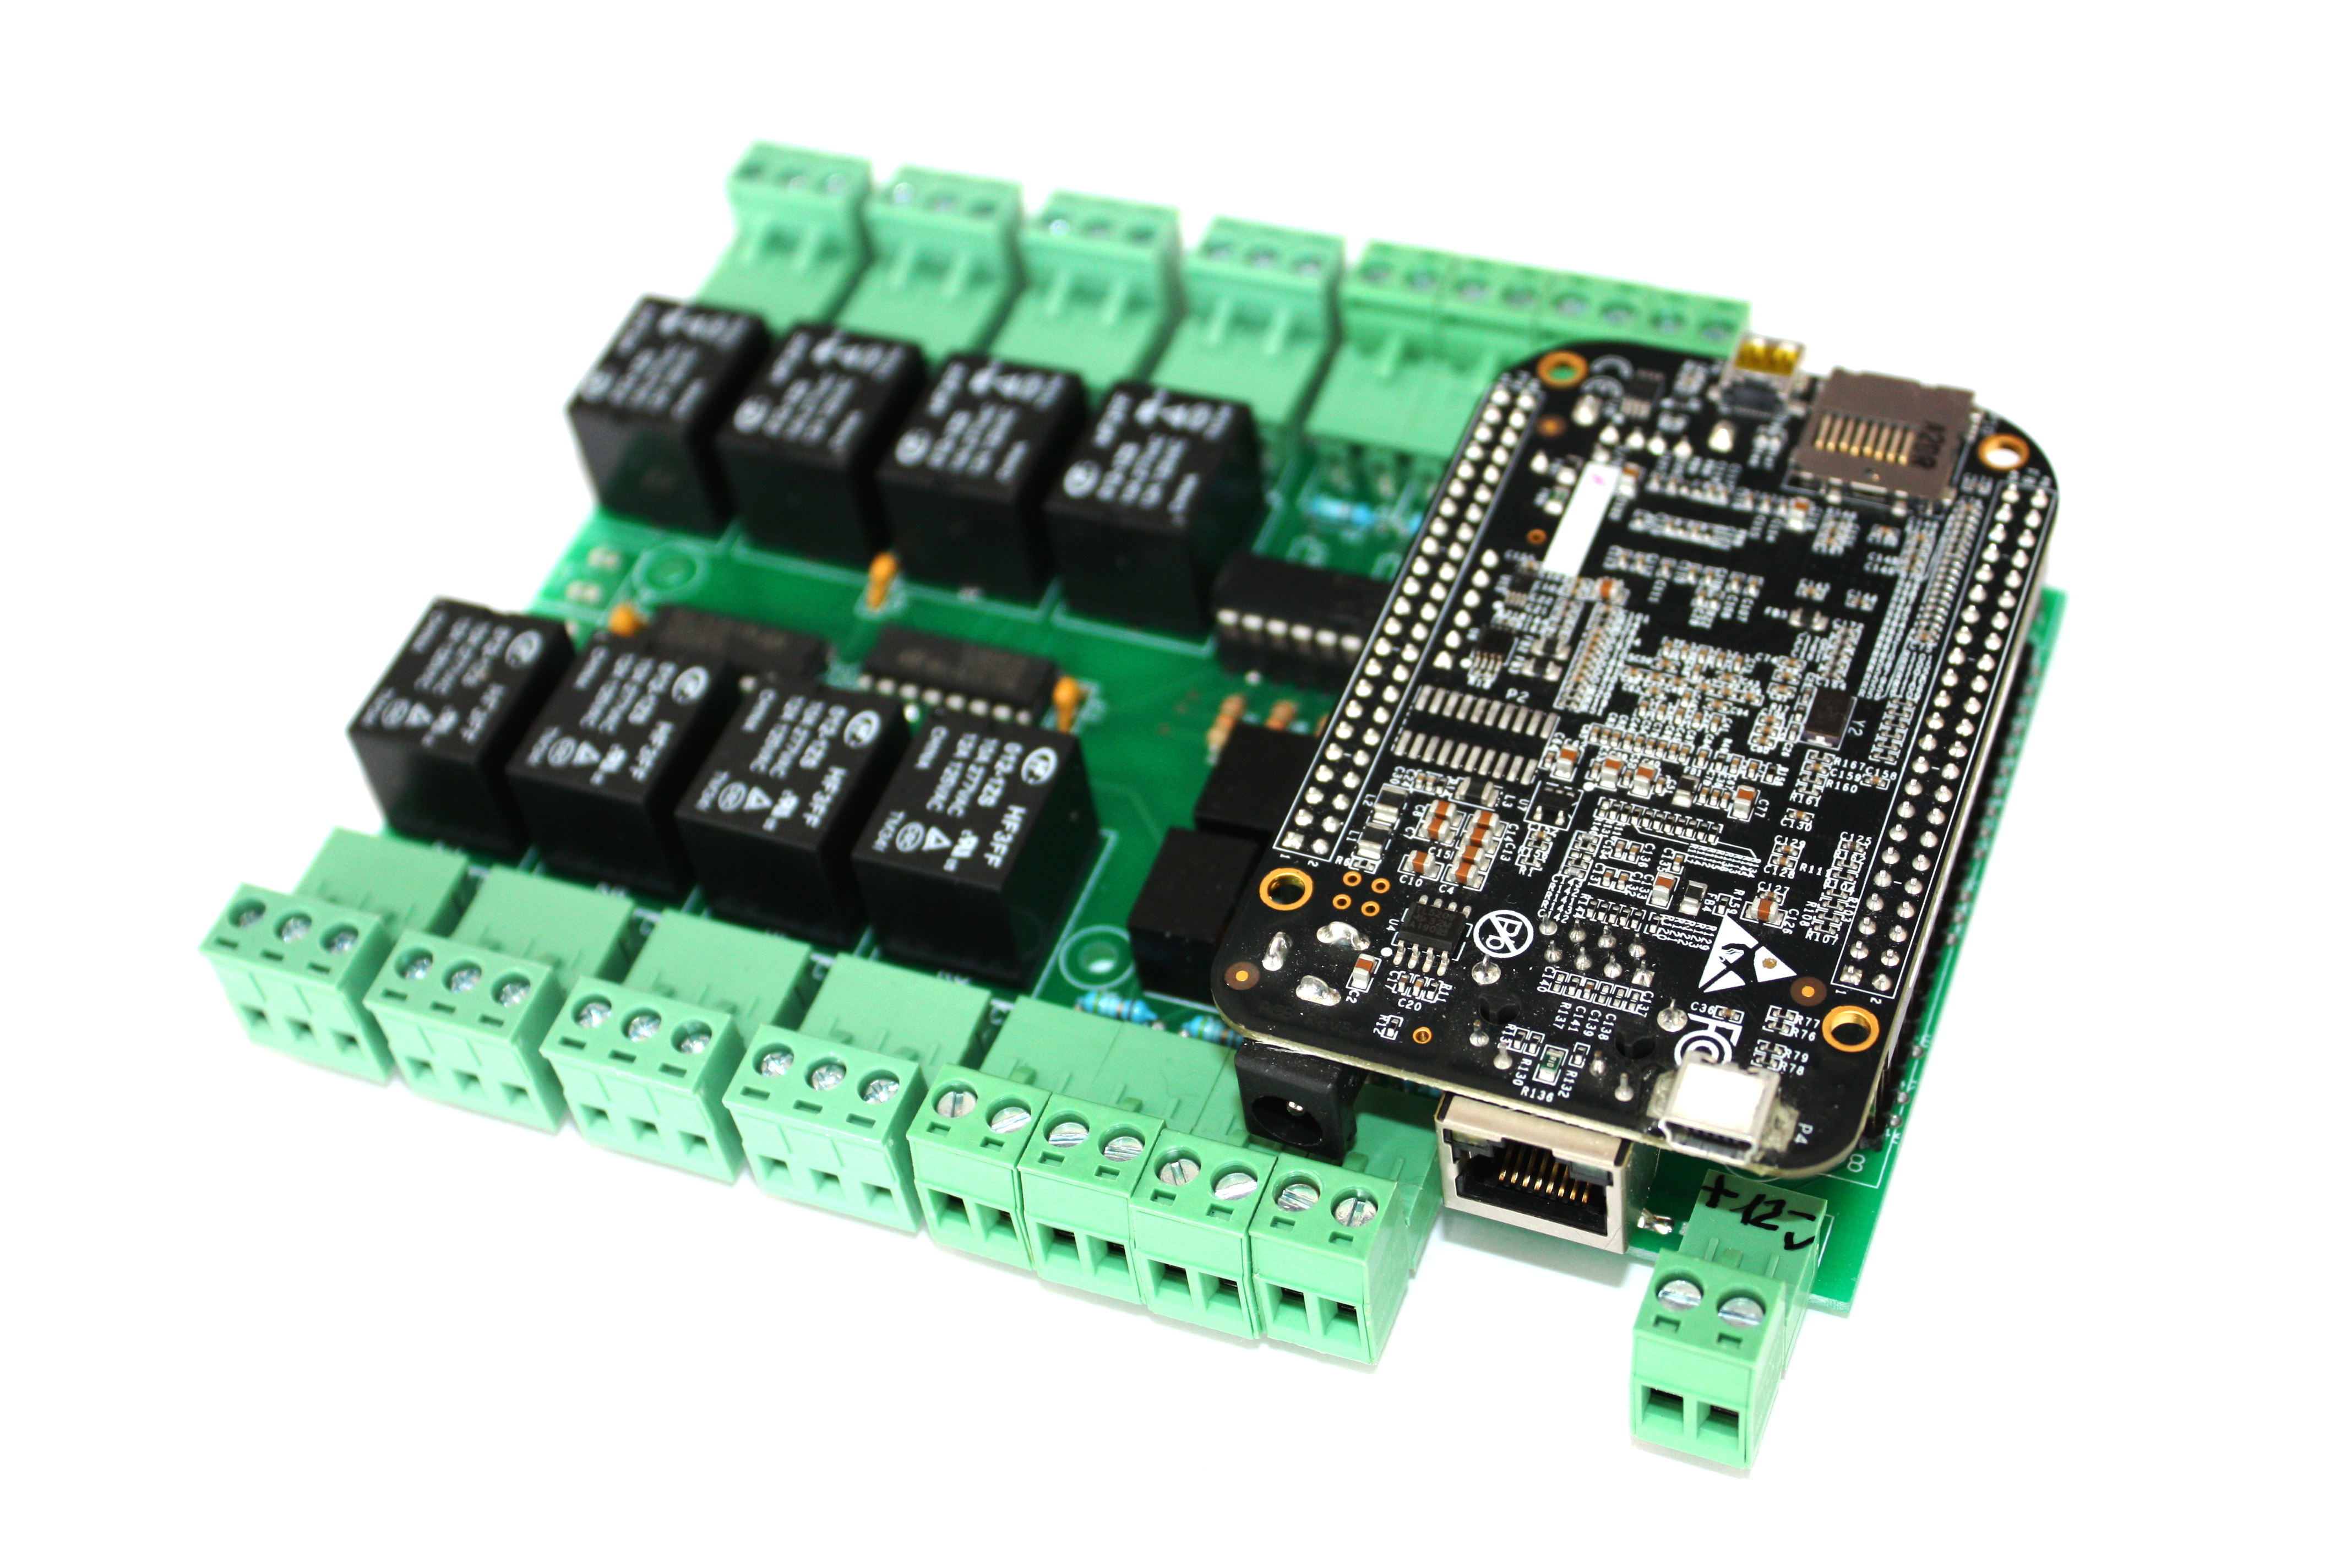
\includegraphics[width=0.75\textwidth,natwidth=585,natheight=180]{assets/images/devices-beaglebone.jpg}
          \caption{BeagleBone Black e OSSO Cape}
          \label{fig:bbb}
        \end{center}
      \end{figure}

      A BeagleBone permite expansões por meio \textit{capes}, placas não-oficiais que permitem melhor explorar o uso das saídas e entradas. Nesse projeto, foi utilizada a OSSO Cape, que dispõe de:

      \begin{itemize}
        \item Oito entradas digitais optoacopladas
        \item Oito saídas digitais por meio de relês
        \item Saída RS-485 integrada
        \item Gerenciamento de fontes externas com tensões entre 5 à 24V
      \end{itemize}

    \subsection{Medidor de Energia Kron Mult-K}

      O medidor de energia é essencial para informar tanto ao usuário, quanto ao sistema central, quanta energia foi consumida durante os carregamentos. O dispositivo escolhido foi o Kron Mult-K, pois esse permite a medição de energia consumida sem a utilização de TCs e os dados são disponibilizados via MODBUS-RTU (conexão RS-485).

      \begin{figure}[H]
        \begin{center}
          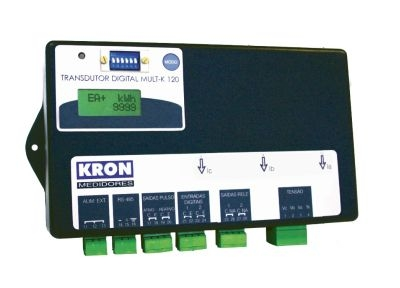
\includegraphics[width=0.75\textwidth,natwidth=400,natheight=288]{assets/images/devices-kron.jpg}
          \caption{Medidor Kron da série Mult-K}
          \label{fig:kron}
        \end{center}
      \end{figure}

    \subsection{Phoenix EM-CP-PP-ETH Controller}

      Os padrões de carregamento rápido utilizam protocolos de comunicação entre carro e estação e, visto a variedade destes, foi escolhido utilizar um controlador externo para agilizar o desenvolvimento do protótipo. O Phoenix EM-CP-PP-ETH permite gerenciar carregamentos AC trifásicos e realizar todo controle necessário para o sequenciamento de inicialização e finalização dos carregamentos.

    \subsection{IHM WEG MT}

      Para o usuário utilizar a \ac{EVSE}, é necessária uma interface que apresente informações de forma descomplicada e, além disso, seja robusta a intempéries como calor excessivo e chuva. Para tal, foi escolhida a \ac{IHM} da WEG, linha MT.

      Utilizando o \textit{software EasyBuilder 8000}, é possível definir as telas que serão exibidas para o usuário, assim como os dados que serão exibidos. Os dados e o controle da IHM podem ser realizados por meio de diversos protocolos, dentre eles o MODBUS-TCP, o qual foi escolhido para o projeto.

      \begin{figure}[H]
        \begin{center}
          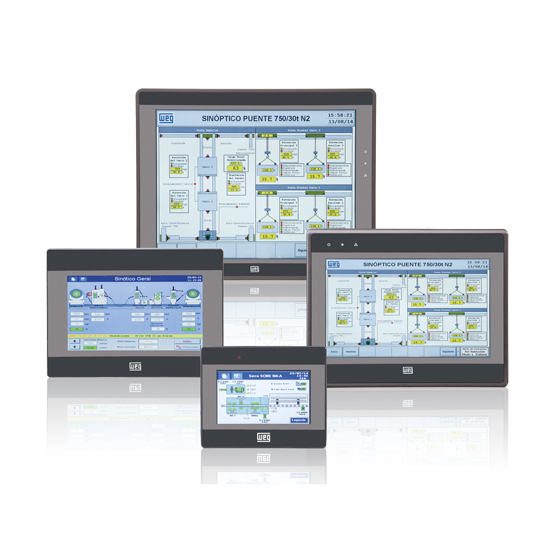
\includegraphics[width=0.75\textwidth,natwidth=400,natheight=288]{assets/images/devices-hmi.jpg}
          \caption{Linha de IHMs MT da WEG}
          \label{fig:ihm}
        \end{center}
      \end{figure}

    \subsection{Leitor de RFID LotusSmart}

      De acordo com a especificação do \ac{OCPP}, para iniciar o carregamento na estação é necessária a utilização de cartões \ac{RFID}, sendo necessário a utilização de um leitor compatível. O dispositivo escolhido, \textit{LotusSmart}, permite apenas a leitura de cartões de 13.56 MHz, visto que há uma variedade de frequências de operação.

      O funcionamento de leitores \ac{RFID} se dá como se fosse um teclado: ao receber os dados do cartão, o leitor envia seus dados para o computador como se esses fossem digitados pelo usuário. Eles são entregues em formato \textit{ASCII}.

      \begin{figure}[H]
        \begin{center}
          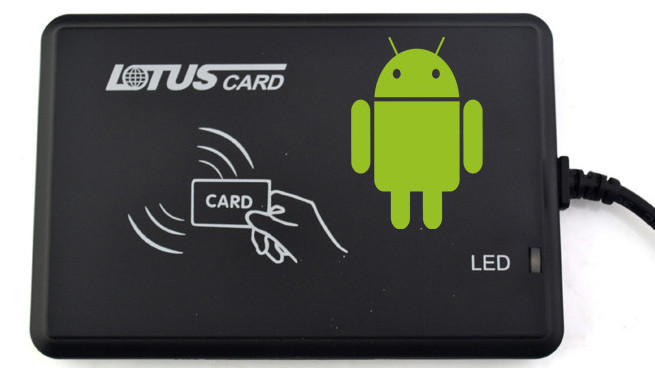
\includegraphics[width=0.75\textwidth,natwidth=655,natheight=368]{assets/images/devices-rfid.jpg}
          \caption{Leitor RFID LotusSmart}
          \label{fig:ihm}
        \end{center}
      \end{figure}

  \section{Métodos e Ferramentas utilizadas}

    \subsection{Protocolo MODBUS}

      Em projetos industriais, é requisito que dispositivos diversos consigam comunicar-se entre si. Para tal, existem dezenas de protocolos que permitem a realização dessa tarefa, sendo o MODBUS um dos mais comuns \cite{modbus-spec-application}. Sua implementação inicial era sob serial, porém hoje também é possível utilizar o stack TCP/IP e outras implementações menos comuns - UDP, PEMEX, Enron.

      \subsubsection{Funcionamento}

        O protocolo é baseado no modelo mestre-escravo, onde um dispositivo mestre requisita os dados dos dispositivos escravos. Essa analogia é muito semelhante ao modelo cliente-servidor, onde o cliente seria o mestre e o servidor o escravo.

        \begin{figure}[H]
          \begin{center}
            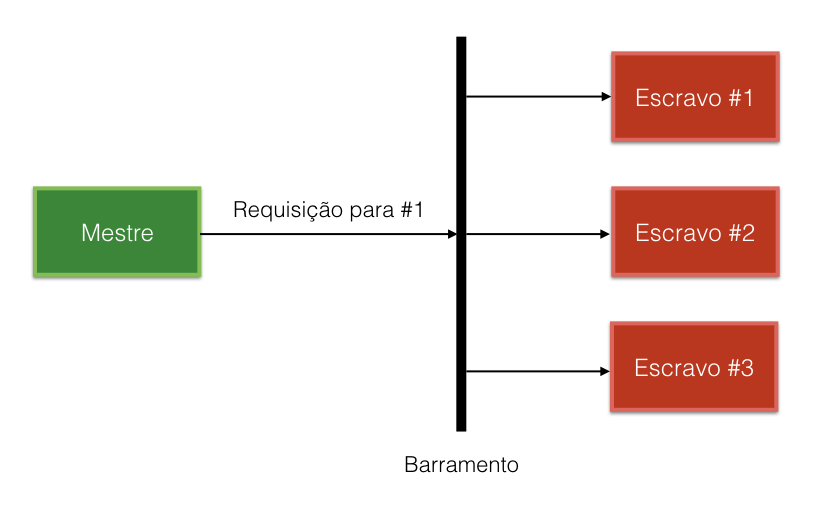
\includegraphics[width=\textwidth,natwidth=1024,natheight=768]{assets/images/modbus-req-1.png}
            \caption{Requisição MODBUS do mestre para o escravo}
            \label{fig:modbus-req-1}
          \end{center}
        \end{figure}

        Como uma rede pode ter N escravos, cada escravo possui um endereço atribuído. O mestre envia a requisição para o barramento e todos os escravos a recebem, porém somente o endereçado responderá. Há também a opção de se fazer um broadcast - endereço 0 - onde todos escravos recebem a requisição, porém nesse caso nenhum escravo deve responde-lá.

        Vale notar que em uma rede MODBUS-RTU há somente um mestre, enquanto em uma rede MODBUS-TCP é possível que cada mestre seja um escravo, e vice-versa.

        \begin{figure}[H]
          \begin{center}
            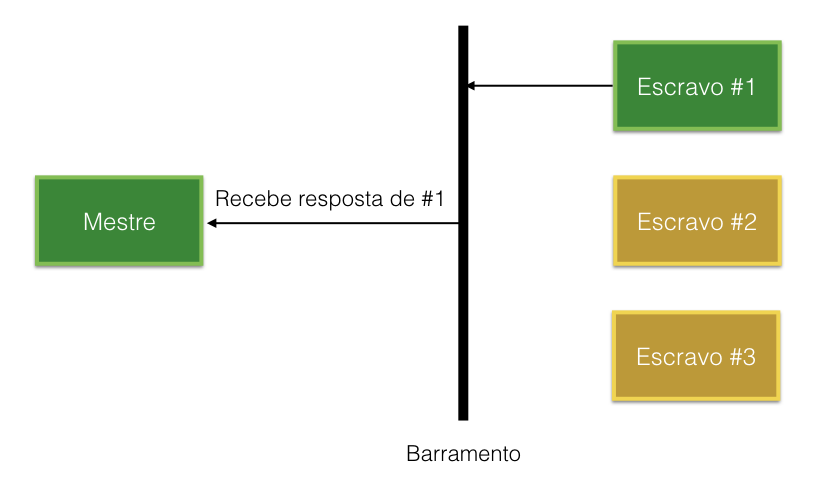
\includegraphics[width=\textwidth,natwidth=1024,natheight=768]{assets/images/modbus-req-2.png}
            \caption{Resposta MODBUS do escravo para o mestre}
            \label{fig:modbus-req-2}
          \end{center}
        \end{figure}

      \subsubsection{Mapa de Memória}

        Toda requisição realizada pelo mestre endereçará um dado no mapa de memória do dispositivo escravo, sendo que tal mapa de memória normalmente deve ser indicado por uma documentação. Os dados requisitados podem possuir quatro tipos distintos:

        \begin{itemize}
          \item \textit{Input}: dado binário que permite apenas leitura
          \item \textit{Coil}: dado binário que permite leitura e escrita
          \item \textit{Input Register}: registrador com 16 bits (inteiro) que permite apenas leitura
          \item \textit{Holding} Register: registrador com 16 bits (inteiro) que permite leitura e escrita
        \end{itemize}

        Para a realização de operações nesse mapa de memória, o mestre precisa informar nas suas requisições um \textit{function code}. Este indicará qual dado deseja-se requisitar e se será executada uma operação de leitura ou escrita. A tabela \ref{table:modbus-funccodes} mostra os mais comuns, porém existem mais códigos, aos quais podem ser usados para diagnósticos e entre outras funções.

        \begin{table}[]
          \centering
          \caption{Function codes / Operações do MODBUS}
          \label{table:modbus-funccodes}
          \begin{tabular}{@{}ll@{}}
            \toprule
            \textbf{Operação}              & \textbf{Function code} \\ \midrule
            Leitura de Coils               & 1                      \\
            Escrita em 1 Coils             & 5                      \\
            Escrita em N Coils             & 15                     \\
            Leitura de Inputs              & 2                      \\
            Leitura de Input Registers     & 4                      \\
            Leitura de Holding Registers   & 3                      \\
            Escrita em 1 Holding Register  & 6                      \\
            Escrita em N Holding Registers & 16                     \\ \bottomrule
          \end{tabular}
        \end{table}

      \subsubsection{Envio de informações}

        Cada modo possui alguma diferença, porém o meio que as informações são organizadas e enviadas é o mesmo. Na imagem a seguir, é possível observar que em ambas implementações é necessária a definição de um \textit{FCode (function code)}. Logo após vem o campo \textit{Data}, onde devem ser indicado o endereço inicial do mapa de memória, quantos registradores deseja-se requisitar e quais dados serão escritos (no caso de escrita).

        \begin{figure}[H]
          \begin{center}
            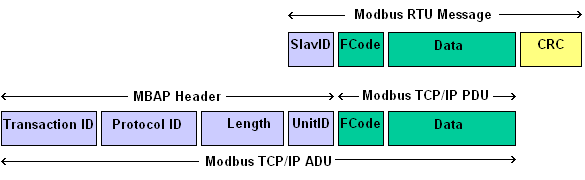
\includegraphics[width=\textwidth,natwidth=585,natheight=180]{assets/images/modbus-frame.png}
            \caption{Frame de Comunicação MODBUS}
            \label{fig:modbus-frame}
          \end{center}
        \end{figure}

        Como pode-se notar, somente no MODBUS-RTU há o SlavID (endereço), já que os dispositivos MODBUS-TCP são endereçados por seus IPs. O campo CRC é um dado que permite checar se o pacote obtido possui ou não algum erro. Como o protocolo TCP/IP já possui um meio para isso, tal campo não é incluído na requisição.

        Esse formato de envio de informações é mantido tanto para requisição quanto para resposta, sendo que as respostas sempre possuem o mesmo \textit{function code} da requisição. Caso diferir, provavelmente ocorreu um erro e este pode ser processado pelo mestre posteriormente.

    \subsection{WSDL e SOAP}

      O WSDL \cite{w3c-spec-wsdl} permite descrever serviços web por meio de um arquivo \ac{XML}. É possível definir os \textit{endpoints} - pontos de entrada para requisições - com o que devem retornar e o que devem receber como parâmetros. Isso permite que um serviço web seja desenvolvido por uma equipe que, posteriormente, exporta um WSDL descrevendo de maneira fácil quais são seus endpoints, facilitando a criação de clientes ou servidores compatíveis com o serviço.

      Os arquivos WSDL definem suas interfaces em SOAP \cite{w3c-spec-soapspec}, um protocolo que permite trocas de informações entre clientes e servidores de forma padronizada. Ele é baseado em XML e é montado em três partes:
      \begin{itemize}
        \item Envolpe: identifica o que é a mensagem e como processá-la
        \item Cabeçalho: define informações extras sobre a mensagem
        \item Corpo: define o procedimento a ser chamado e os dados de sua resposta
      \end{itemize}

      Como ele foi idealizado em XML, ele é facilmente processado por qualquer linguagem de programação, o que garante uma boa portabilidade.

  \section{Estrutura do Projeto}

    A figura \ref{fig:proj-diagram} apresenta o diagrama de conexão dos dispositivos. Como todos os dispositivos são compatíveis com MODBUS, esse foi o protocolo escolhido para a comunicação entre eles. Para a comunicação entre servidor e estação, foi escolhido o protocolo \ac{OCPP} 1.5.

    A estação possui dois medidores, sendo um de carregamento normal/lento e outro de carregamento rápido. Cada conector possui seu próprio medidores de energia, porém seus controles se dão de forma diferente: o de carregamento rápido utiliza o controlador Phoenix, enquanto o conector normal é controlado pela \textit{BeagleBone} e um relê, visto que ele é somente uma tomada comum e não necessita de nada muito elaborado para inicializar carregamentos (diferente do rápido, onde há um protocolo entre estação e carro).

    \begin{figure}[H]
      \begin{center}
        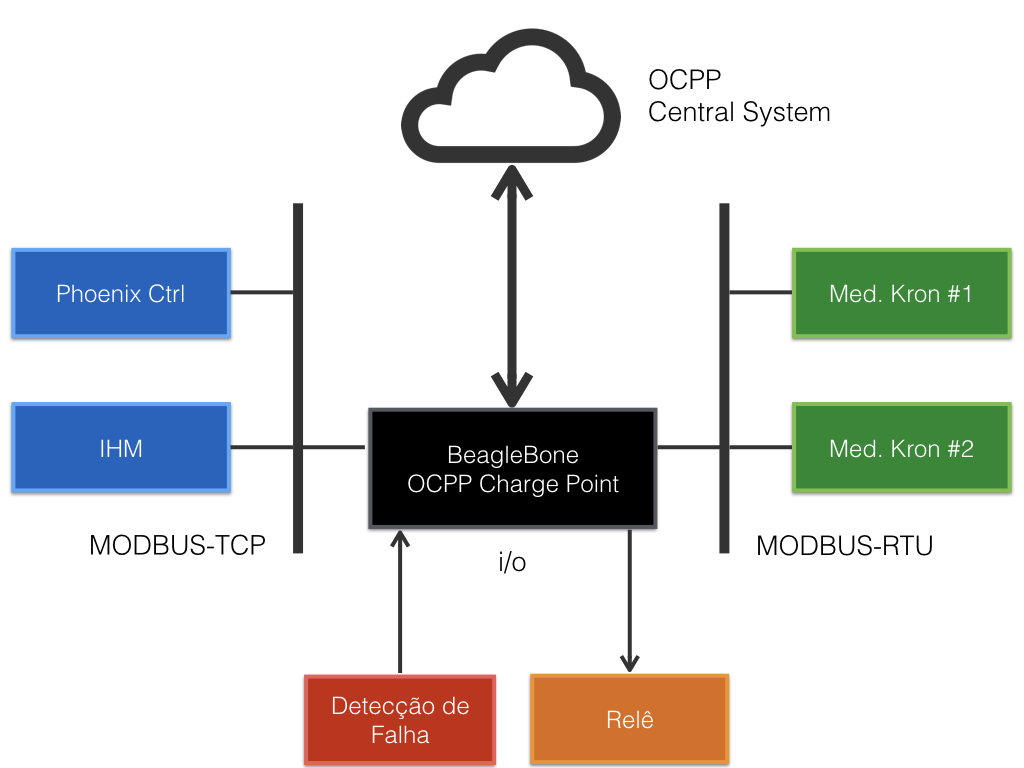
\includegraphics[width=0.8\textwidth,natwidth=400,natheight=288]{assets/images/devices-diagram.png}
        \caption{Diagrama de conexão entre os dispositivos da \ac{EVSE}}
        \label{fig:proj-diagram}
      \end{center}
    \end{figure}

    \subsection{Sistema Operacional}

      O sistema que roda na BeagleBone é o Debian 8.6 (Jessie) com kernel Linux específico para a \textit{BeagleBone}. Foi instalado o Java 1.7 e houveram modificações em sua \textit{device tree} para permitir a manipulação das entradas e saídas digitais.

      Foram adicionados alguns scripts ao boot do sistema para ativar o acesso à internet e executar o programa logo após a inicialização do sistema.

    \subsection{Comunicação entre periféricos}

      Visto que todos dispositivos escolhidos suportam MODBUS, esse foi o protocolo escolhido como padrão. A biblioteca \textit{Jamod} foi utilizada para realizar a implementação do protocolo no projeto.

    \subsection{Comunicação entre estação e servidores}

      A estação implementa o protocolo \ac{OCPP} 1.5, ao qual é suportado por outras estações comerciais vendidas no Brasil, permitindo comunicação com equipamentos e \textit{softwares} já existentes. A \ac{OCA}, responsável pelo protocolo, disponibiliza um arquivo WSDL, onde é possível criar tanto um servidor quanto um cliente OCPP facilmente.

      Para a utilização desse arquivo em Java, foi utilizada a ferramenta \textit{wsimport}. Ela importa os arquivos e cria classes \textit{Java} correspondentes a cada \textit{endpoint}. Nem todas funções especificadas pelo protocolo foram implementadas, sendo somente as da tabela \ref{table:ocpp} são suportadas.

      \begin{table}[]
        \centering
        \caption{Operações OCPP suportadas pela \ac{EVSE}}
        \label{table:ocpp}
        \begin{tabular}{@{}ll@{}}
          \toprule
          \textbf{Enviada/Recebida} & \textbf{Operação}      \\ \midrule
            Enviada pela Estação      & BootNotification       \\
            Enviada pela Estação      & Heartbeat              \\
            Enviada pela Estação      & StartTransaction       \\
            Enviada pela Estação      & StopTransaction        \\
            Enviada pela Estação      & MeterValues            \\
            Enviada pela Estação      & StatusNotification     \\
            Enviada pela Estação      & Authorize              \\
            Recebida pela Estação     & RemoteStartTransaction \\
            Recebida pela Estação     & RemoteStopTransaction  \\
            Recebida pela Estação     & ChangeConfiguration    \\
            Recebida pela Estação     & GetConfiguration       \\
            Recebida pela Estação     & ChangeAvailability     \\ \bottomrule
        \end{tabular}
      \end{table}

    \subsection{IHM e do sistema central}

      O desenvolvimento da IHM e do sistema central não foi desenvolvido pelo acadêmico, porém são de importância fundamental para o projeto.

    \subsection{Software}

      O software foi desenvolvido em Java [...]

  \section{Testes}

    \subsection{Ferramentas de teste}

      Para testar a implementação realizada, é necessária uma ferramenta para simular um servidor central. Inicialmente, testou-se a ferramenta \textit{OCPPJS} (http://www.gir.fr/ocppjs/), porém essa apresentou problemas ao lidar com algumas das requisições vindas da \ac{EVSE}.

      Foi criada então uma ferramenta para testes, disponível no \textit{Github} (https://github.com/brnluiz/ocpp-tools), que implementa parcialmente as funções de um sistema central. Todas operações apresentadas na tabela \ref{table:ocpp} foram implementadas.

      Após aberta, a ferramenta ouvirá todas requests das estações que estiverem conectadas à ela e responderá com dados genéricos, possibilitando o funcionamento da estação. Caso o desenvolvedor precise executar alguma requisição às estações, é possível utilizar a \ac{CLI} para tal (os comandos disponíveis são dados pelo manual da ferramenta).

    \subsection{Implementações e testes iniciais}

      O desenvolvimento inicial se deu no estudo da base de código anterior, que ainda não implementava nada da \ac{EVSE} funcionalmente, apenas possibilitava o teste de cada dispositivo isoladamente. Após esse período inicial, deu-se a implementação do software da estação.

      Alguns testes unitários foram desenvolvidos sob o framework de testes \textit{JUnit}, o que permite o programa ser testado antes de ser embarcado. Assim que todos testes passam, o programa é enviado para a \textit{BeagleBone}.

      Como as cargas utilizadas durante o teste consumiam pouca energia (fontes AC-DC de dispositivos como notebooks), o medidor de energia teve seu multiplicador de corrente configurado em 100, possibilitando assim simular um consumo alto de forma rápida (sem ter que aguardar várias horas para chegar em 1kWh).

      Todos arquivos, incluindo o sistema operacional, são colocados no cartão SD, o que facilita a cópia desses dados para backup (criação de imagens) e permite o intercâmbio do sistema entre a bancada de testes e a estação protótipo.

      \begin{figure}[H]
        \begin{center}
          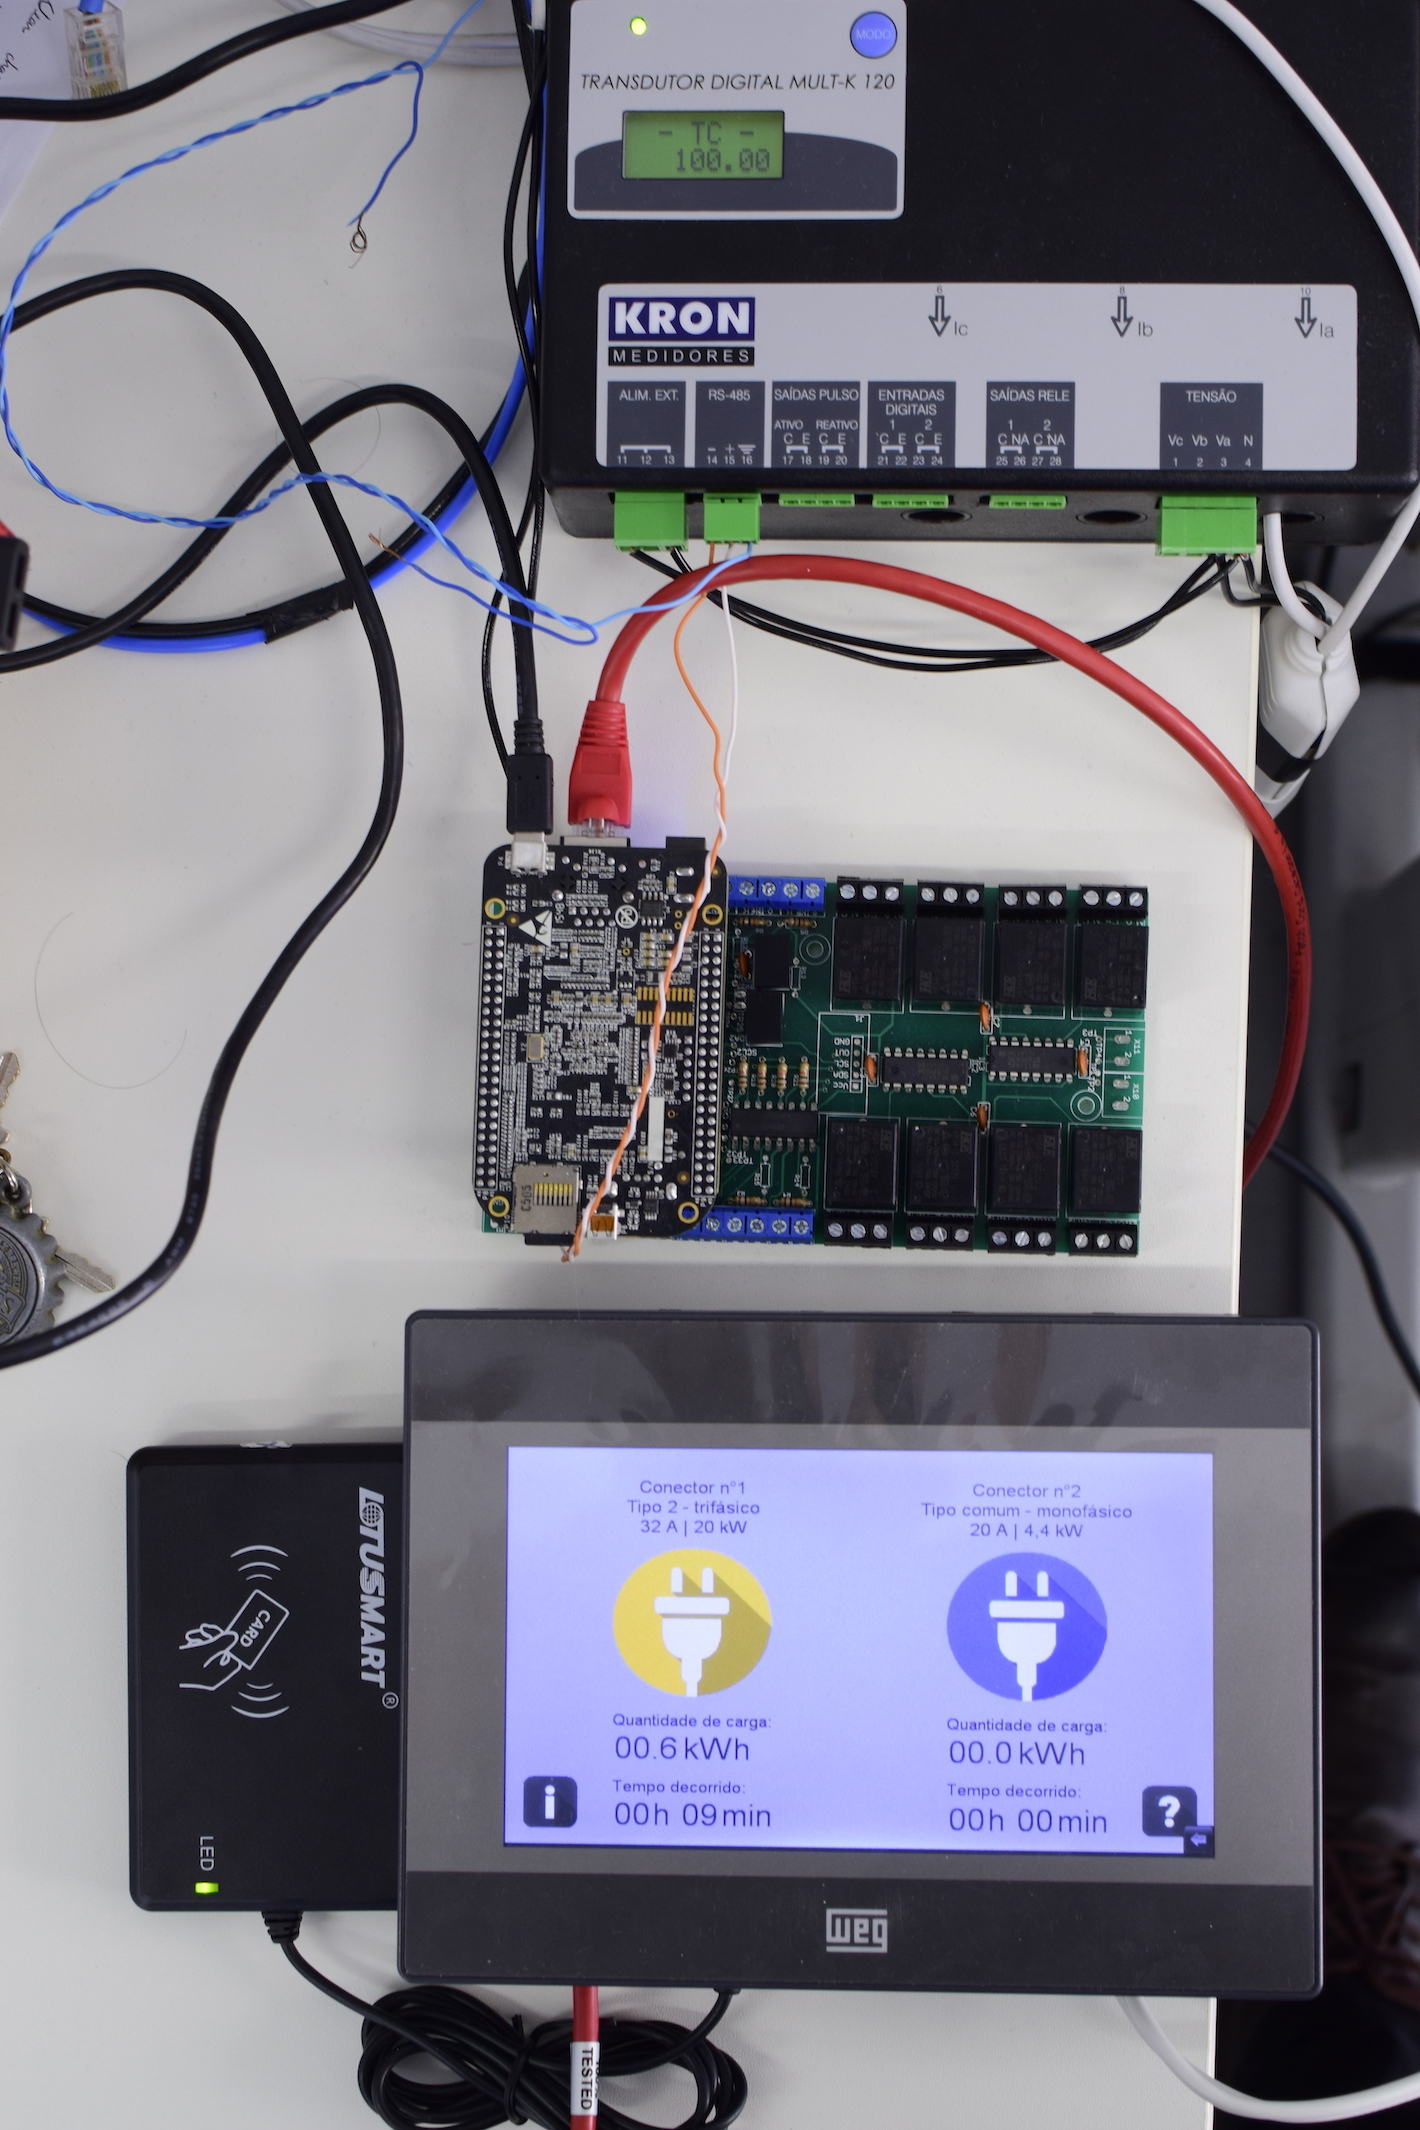
\includegraphics[width=0.6\textwidth,natwidth=2130,natheight=1420,angle=-90]{assets/images/prototype-setup.jpg}
          \caption{Disposição dos dispositivos na bancada de testes}
          \label{fig:prototype-setup}
        \end{center}
      \end{figure}

    \subsection{Testes na estação protótipo}

      Após diversos testes na configuração mostrada na figura \ref{fig:prototype-setup}, o sistema foi levado para a estação protótipo, situada no estacionamento da Fundação CERTI. A disposição dos dispositivos da estação difere com a da bancada de testes, porém visto que os dispositivos são os mesmos e o sistema embarcado foi colocado em um cartão SD, só é necessário inserir o cartão na BeagleBone da estação e configurá-la para dar boot pelo cartão, caso já não estiver configurada por fábrica assim.

      \begin{figure}[H]
        \begin{center}
          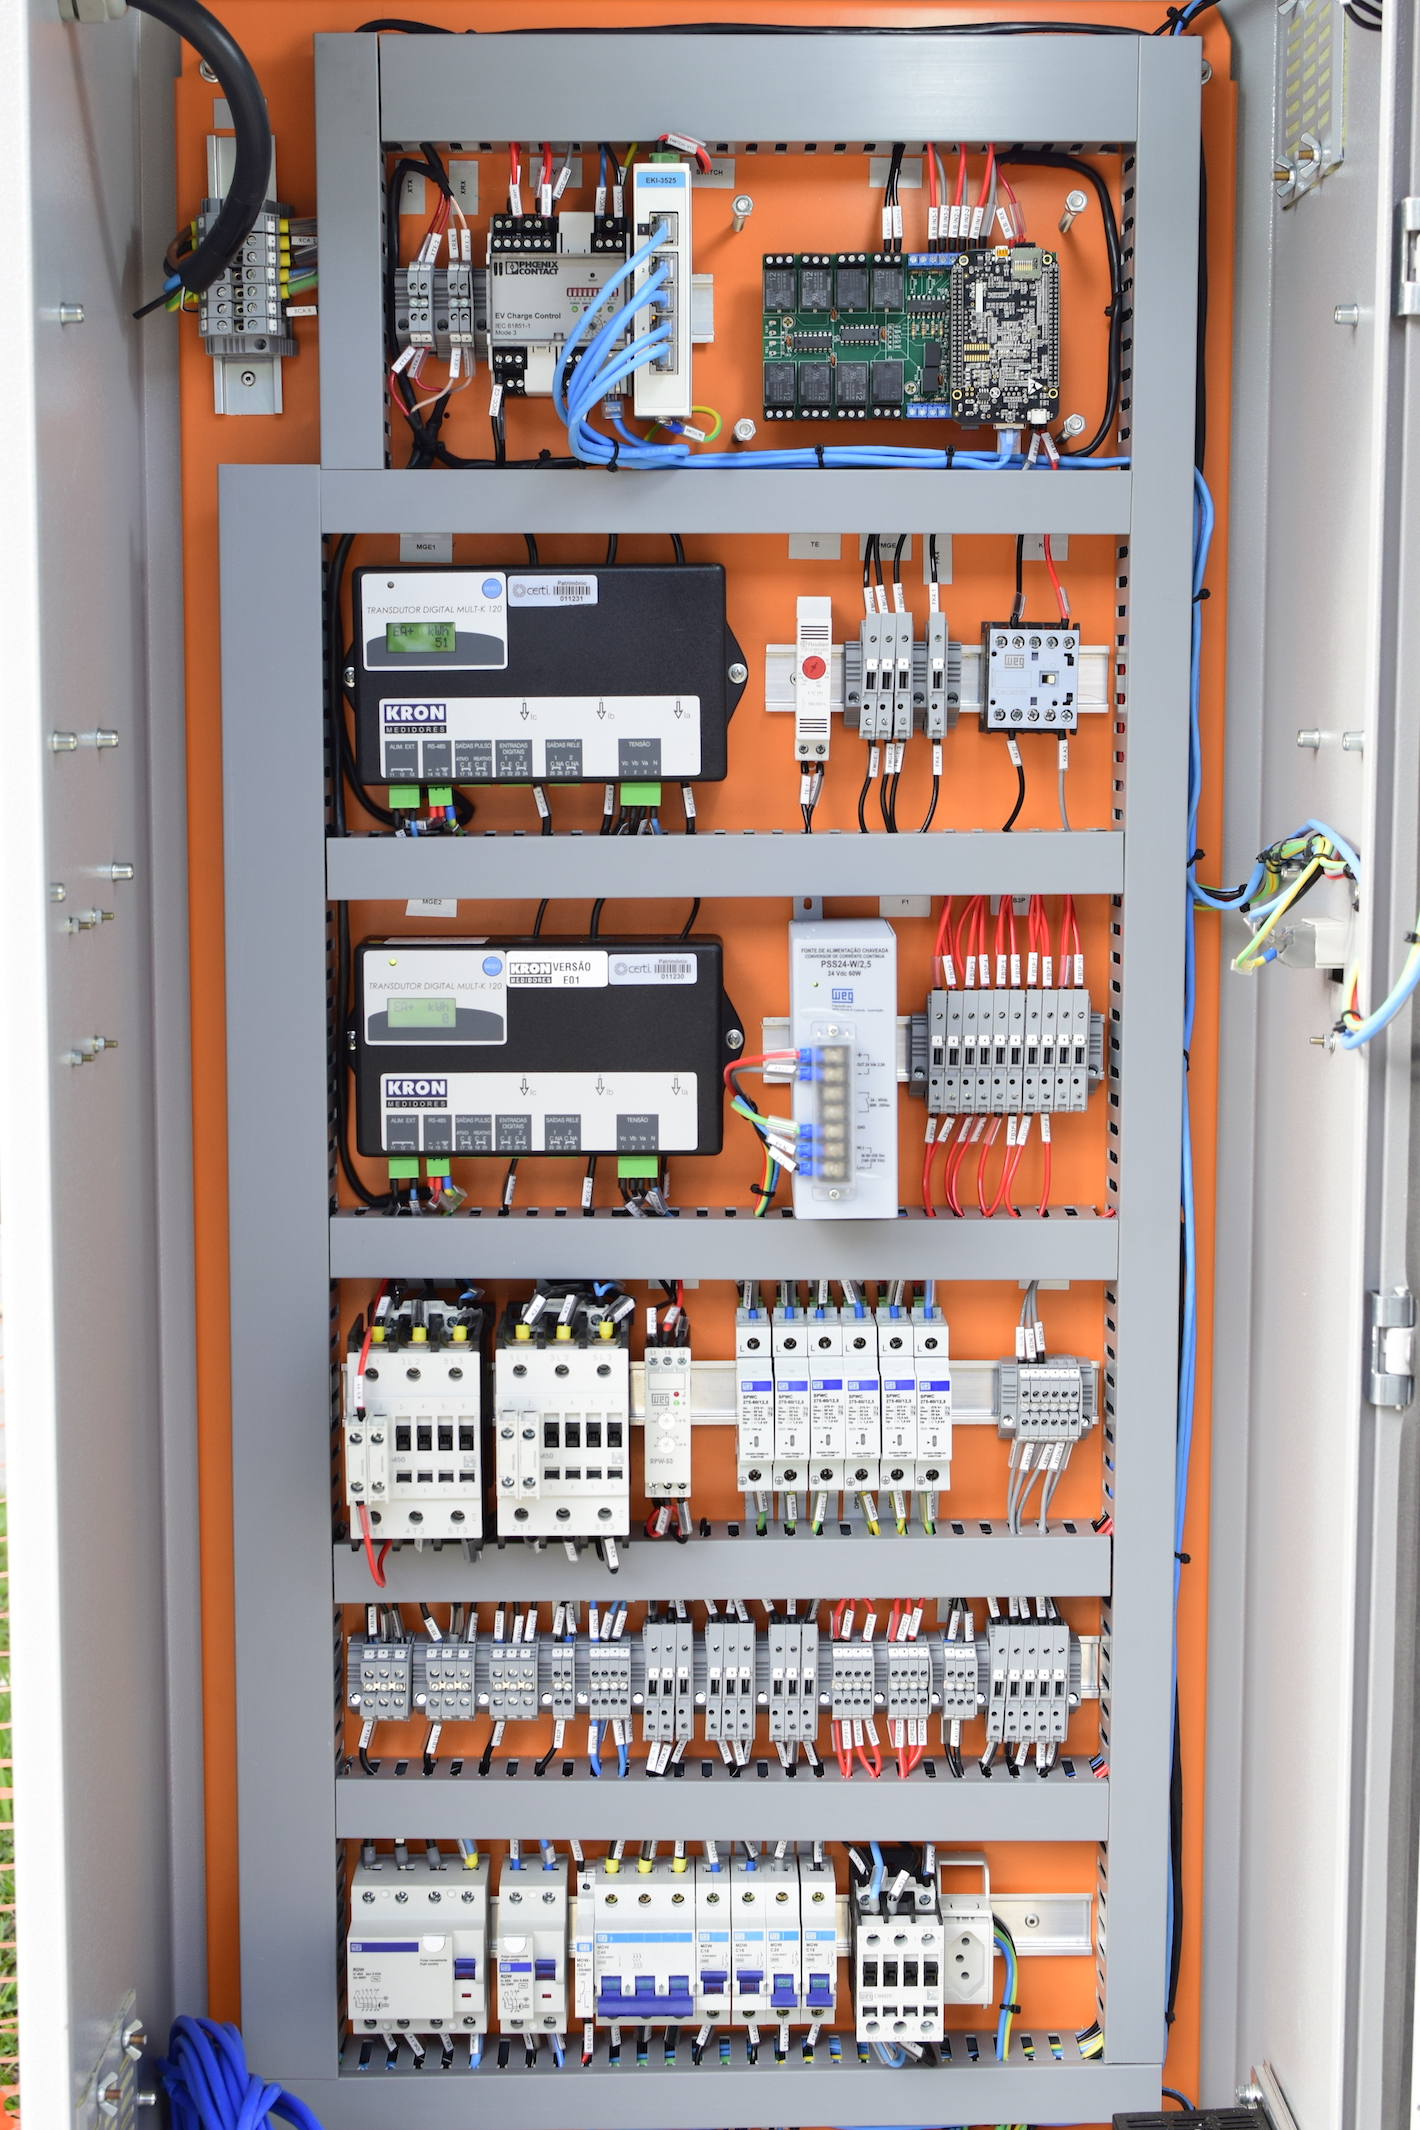
\includegraphics[width=\textwidth,natwidth=1420,natheight=2130]{assets/images/evse-setup.jpg}
          \caption{Disposição dos dispositivos na estação protótipo}
          \label{fig:evse-setup}
        \end{center}
      \end{figure}
